\documentclass{article}

\usepackage{graphicx}
\usepackage{listings}
\usepackage[T1]{fontenc}

\newcommand{\bslash}{\char`\\}

\title{Assignment 1: Design}
\date{3 Feb -- Winter 2017}
\author{Jeremiah Griffin}

\begin{document}

  \lstset{
    language=C++,
    basicstyle=\ttfamily
  }

  % Title page
  \pagenumbering{gobble}
  \maketitle
  \newpage
  \pagenumbering{arabic}

  % Introduction
  \section{Introduction}

  In this project I will design a basic POSIX command shell using the
  composite and strategy patterns with a strong emphasis on object
  oriented design principles and correctness.  This design separates the
  semantic structure of commands from its model of execution and allows
  the user a high degree of composability while simultaneously leaving
  the design of the system open for future extensions wherein the
  developer might create a more feature-complete shell.  The classes set
  forth in this design use language constructs intended to ensure that
  sensible invariants are necessarily preserved at all times, making it
  largely impossible to create an invalid object graph in the domain of
  the design.

  The operation of this design is in a loop, the body of which is as
  follows:

  \begin{enumerate}
    \item The \texttt{Shell} instance prompts the user for a command.
    \item The provided command is tokenized by the
      \texttt{Tokenizer} class.
    \item The command tokens are parsed into one or more
      \texttt{Command} instances using the composite pattern to
      represent chained commands and their conditions.
    \item The \texttt{Command} instance is given to an
      \texttt{Execution}.
    \item The \texttt{Execution} processes each \texttt{Command} in the
      composition using its \texttt{Executor}, which is instantiated
      according to the underlying operating system and performs the
      necessary platform-specific operations to execute the given
      command.
  \end{enumerate}

  % Diagram
  \section{Diagram}

  \includegraphics[page=2,scale=0.6]{Diagram.pdf}
  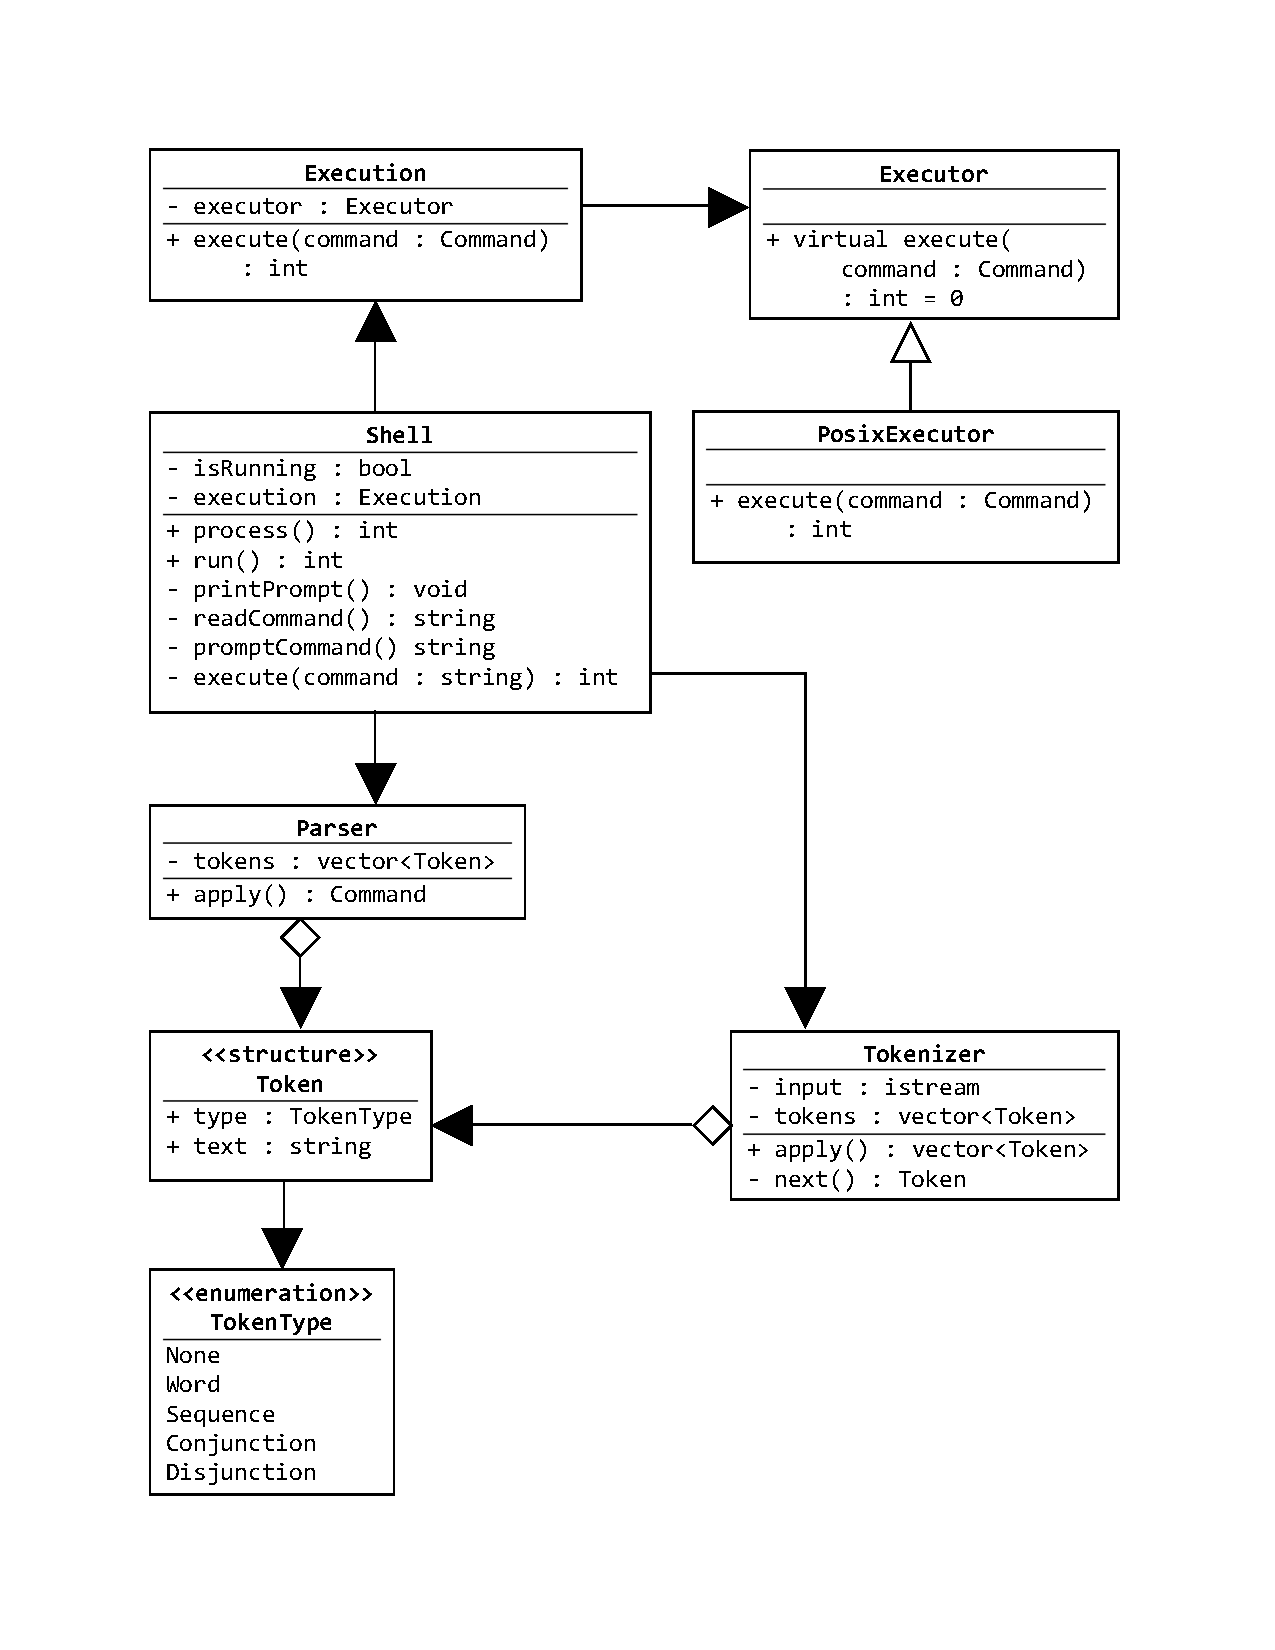
\includegraphics[page=1,scale=0.6]{Diagram.pdf}

  % Classes
  \section{Classes}

  \subsection{\texttt{Shell}}

  This is the class which presents a user-friendly interface and
  provides the point of interaction for accepting and executing user
  commands.  It is responsible for instantiating an appropriate
  \texttt{Execution}, printing command prompts, accepting commands,
  tokenizing and parsing command strings into \texttt{Command}
  instances, and offering commands for execution.

  The command string input process allows for multiline commands.  If a
  command ends with a backslash or in the middle of a quoted string, the
  continuation prompt is printed and another line of input is accepted,
  appended to the command string.  If the previous line terminated with
  a backslash, the next line is joined to the command string directly.
  If the previous line was terminated in the middle of a quoted string,
  the next line is joined with a line terminator.

  \subsubsection{Interface}
  \lstinputlisting[firstline=1,lastline=19]{Interfaces.hpp}

  \subsubsection{Members}
  \begin{itemize}
    \item \texttt{isRunning}: Whether or not the shell is running.  This
      will be set to false when the \texttt{exit} command is received.
    \item \texttt{execution}: The execution instance to used for
      executing commands.
  \end{itemize}

  \subsubsection{Methods}
  \begin{itemize}
    \item \texttt{process}: Prompts for, reads, and executes a command.
    \item \texttt{run}: Repeatedly calls \texttt{process} as long as
      \texttt{isRunning} is true.
    \item \texttt{printCommandPrompt}: Prints the prompt to begin a
      command.
    \item \texttt{printContinuationPrompt}: Prints the prompt to
      continue a command.
    \item \texttt{readCommand}: Reads a command string from the standard
      input, prompting for continuation as necessary.
    \item \texttt{promptCommand}: Prompts for and reads a command string.
    \item \texttt{execute}: Tokenizes, parses, and executes the given
      command string.
  \end{itemize}

  \subsection{\texttt{Token}}

  This structure represents a lexical token within a command string,
  such as a command word or chaining connective.

  \subsubsection{Interface}
  \lstinputlisting[firstline=21,lastline=34]{Interfaces.hpp}

  \subsubsection{Enumerations}
  \begin{itemize}
    \item \texttt{Token}: The types of tokens that may appear in a
      command string.
      \begin{itemize}
        \item \texttt{None}: Represents the end of a token stream.
        \item \texttt{Word}: A space-delimited word or quoted grouping
          of words.
        \item \texttt{Sequence}: A sequenced command delimiter (;).
        \item \texttt{Conjunction}: A conjoined command delimiter (\&\&).
        \item \texttt{Disjunction}: A disjoined command delimiter (||).
      \end{itemize}
  \end{itemize}

  \subsubsection{Members}
  \begin{itemize}
    \item \texttt{type}: The enumerated type of the token.
    \item \texttt{text}: The body text of the token.
  \end{itemize}

  \subsection{\texttt{Tokenizer}}

  This class accepts a string and transforms it into a stream of
  \texttt{Token} instances through lexical analysis.  The
  classifications used in this analysis are represented with the
  following regular expressions, in the order of descending precedence,
  where the \bslash s sequence represents a white-space character and
  each expression is surrounded by any number of white-space characters
  on either side:

  \lstinputlisting[language=]{Language.txt}

  During this process, escaped sequences are processed and replaced with
  the appropriate character, as defined in the following mapping:

  \begin{tabular}{l|l}
    Sequence & Substitution \\
    \hline
    \bslash a & Bell \\
    \bslash e & Escape \\
    \bslash n & Line feed \\
    \bslash r & Carriage return \\
    \bslash t & Tab \\
    \bslash \emph{char} & \emph{char}
  \end{tabular}

  The last substitution in the table above allows for the insertion of
  quotes, backslashes, and other special characters as elements of a
  word.

  \subsubsection{Interface}
  \lstinputlisting[firstline=36,lastline=50]{Interfaces.hpp}

  \subsubsection{Members}
  \begin{itemize}
    \item \texttt{input}: The input stream to tokenize.
    \item \texttt{tokens}: The produced sequence of tokens.
  \end{itemize}

  \subsubsection{Methods}
  \begin{itemize}
    \item \texttt{apply}: Repeatedly tokenizes until the end of the
      input stream is reached, returning the produced tokens.
    \item \texttt{next}: Obtains the next token from the stream.  If
      there are no more tokens available, the returned token will have
      the \texttt{None} type.
  \end{itemize}

  \subsection{\texttt{Parser}}

  This class accepts a sequence of tokens and transforms it into a chain
  of one or more commands, provided that the token stream meets the
  grammatical requirements of a command, as defined in the following
  recursive grammar notated in extended Backus-Naur form, using the
  expressions defined in the language of the \texttt{Tokenizer} class:

  \lstinputlisting[language=]{Grammar.ebnf}

  \subsubsection{Interface}
  \lstinputlisting[firstline=52,lastline=61]{Interfaces.hpp}

  \subsubsection{Members}
  \begin{itemize}
    \item \texttt{tokens}: The sequence of tokens to parse as a command.
  \end{itemize}

  \subsubsection{Methods}
  \begin{itemize}
    \item \texttt{apply}: Parses the token sequence according to the
      defined grammar and returns the resultant command.  If the
      sequence is not well-formed, a null pointer is returned.
  \end{itemize}

  \subsection{\texttt{Command}}

  This class serves as the abstract base class in the composite pattern
  of the command structure.  It represents a polymorphic command to be
  executed.

  \subsubsection{Interface}
  \lstinputlisting[firstline=93,lastline=104]{Interfaces.hpp}

  \subsubsection{Members}
  \begin{itemize}
    \item \texttt{program}: The name of the program to execute.
    \item \texttt{arguments}: The arguments to pass to the program upon
      execution.
    \item \texttt{next}: The next command to execute within the chain,
      if any.
  \end{itemize}

  \subsubsection{Methods}
  \begin{itemize}
    \item \texttt{shouldExecuteAfter}: Returns true if this command
      should be executed after the given command, which exited with the
      provided code upon completion.
  \end{itemize}

  \subsection{\texttt{InitialCommand}}

  The first command within a command chain.

  \subsubsection{Interface}
  \lstinputlisting[firstline=106,lastline=115]{Interfaces.hpp}

  \subsubsection{Methods}
  \begin{itemize}
    \item \texttt{shouldExecuteAfter}: Returns false, as an initial
      command should never be executed after another command.
  \end{itemize}

  \subsection{\texttt{SequentialCommand}}

  A command to be executed unconditionally within a command chain.

  \subsubsection{Interface}
  \lstinputlisting[firstline=115,lastline=122]{Interfaces.hpp}

  \subsubsection{Methods}
  \begin{itemize}
    \item \texttt{shouldExecuteAfter}: Returns true, as a sequential
      command is always executed.
  \end{itemize}

  \subsection{\texttt{ConjunctiveCommand}}

  A command to be executed if the preceding command exited successfully
  with a zero exit code.

  \subsubsection{Interface}
  \lstinputlisting[firstline=124,lastline=131]{Interfaces.hpp}

  \subsubsection{Methods}
  \begin{itemize}
    \item \texttt{shouldExecuteAfter}: Returns true if the exit code is
      zero.
  \end{itemize}

  \subsection{\texttt{DisjunctiveCommand}}

  \subsubsection{Interface}
  \lstinputlisting[firstline=133,lastline=140]{Interfaces.hpp}

  A command to be executed if the preceding command exited
  unsuccessfully with a nonzero exit code.

  \subsubsection{Methods}
  \begin{itemize}
    \item \texttt{shouldExecuteAfter}: Returns true if the exit code is
      nonzero.
  \end{itemize}

  \subsection{\texttt{Execution}}

  This class represents the algorithm for executing commands in the
  strategy pattern.  It continues to execute subsequent commands in a
  chain as long as the \texttt{shouldExecuteAfter} continues to return
  true given the results of the preceding command.  It uses its internal
  \texttt{Executor} instance to perform the actual execution of
  commands.

  \subsubsection{Interface}
  \lstinputlisting[firstline=63,lastline=75]{Interfaces.hpp}

  \subsubsection{Members}
  \begin{itemize}
    \item \texttt{executor}: The executor to perform the execution of
      commands with.
  \end{itemize}

  \subsubsection{Methods}
  \begin{itemize}
    \item \texttt{execute}: Executes the given command structure using
      the algorithm given above.  If at any point a command with the
      program name "exit" is given and meant to be executed, an
      exception is thrown, intending to signal to the caller that no
      more commands should be processed and the shell should terminate.
      Returns the exit code of the last command executed.
  \end{itemize}

  \subsection{\texttt{Executor}}

  This class serves as the abstract base class in the strategy pattern
  of the execution algorithm.  It represents a polymorphic function to
  perform the actual execution of a single command.

  \subsubsection{Interface}
  \lstinputlisting[firstline=77,lastline=83]{Interfaces.hpp}

  \subsubsection{Methods}
  \begin{itemize}
    \item \texttt{execute}: Executes the individual command given and
      returns its exit code.
  \end{itemize}

  \subsection{\texttt{PosixExecutor}}

  This class implements the execution algorithm by executing commands
  through POSIX system calls.

  \subsubsection{Interface}
  \lstinputlisting[firstline=85,lastline=91]{Interfaces.hpp}

  \subsubsection{Methods}
  \begin{itemize}
    \item \texttt{execute}: Executes the individual command given and
      returns its exit code.
  \end{itemize}

  % Coding Strategy
  \section{Coding Strategy}

  I am working without a partner, thus there is no per-person division
  of work.  Instead, I will describe the order in which I will implement
  the components of the system.  My goal is to have a reasonably
  functional program after each stage.

  \begin{enumerate}
    \item \texttt{Command} class
    \item \texttt{InitialCommand} class
    \item \texttt{SequentialCommand} class
    \item \texttt{ConjunctiveCommand} class
    \item \texttt{DisjunctiveCommand} class
    \item \texttt{Token} structure
    \item \texttt{Tokenizer} class
    \item \texttt{Parser} class
    \item \texttt{Executor} class
    \item \texttt{PosixExecutor} class
    \item \texttt{Execution} class
    \item \texttt{Shell} class
  \end{enumerate}

  % Roadblocks
  \section{Roadblocks}

  For this assignment, the design is reasonably well-defined, and I do
  not foresee any roadblocks in its implementation.  However, there
  could potentially be issues inherent to the design that hamper the
  extensibility of the system.

  A common feature of shells is builtin commands, such as \texttt{alias}
  in bash and zsh.  To implement these, the most straightforward
  approach in this system is to write a new executor type,
  \texttt{BuiltinExecutor}, which performs the processing.  However,
  this would lead to problems when builtin commands are chained with
  external commands.  To solve this, a system would need to be created
  to select an executor on a per-command basis.  This might be
  accomplished using a set of \texttt{Executor} instances in the
  \texttt{Execution}, which then delegates work to the appropriate
  executor depending on the nature of each \texttt{Command}.

  Another feature that is not directly addressed in this specification
  is command comments, which are necessary for this assignment.  A
  likely point of implementation for this feature is within the
  \texttt{Tokenizer} class, whose language could be extended to discard
  all characters after a comment token.

\end{document}
